\documentclass[11pt,a4paper]{article}

\usepackage[polish]{babel}
\usepackage[utf8]{inputenc}
\usepackage{polski}
\usepackage[T1]{fontenc}
\usepackage{indentfirst}
\usepackage{wrapfig}    % for wrapping figures, tables

\frenchspacing

%\usepackage{amsmath}
\usepackage{physics}
%\usepackage{bm}
\usepackage{gensymb}
%\usepackage{hepnames}
\usepackage{epsfig}
\usepackage{graphics}
\usepackage[shortlabels]{enumitem}
%\usepackage{xspace}
%\xspaceaddexceptions{[]\{\}}

%
%
%fixpagesize
\pagestyle{empty}
\addtolength{\textwidth}{6cm}
\addtolength{\textheight}{4cm}
\addtolength{\evensidemargin}{-3cm}
\addtolength{\oddsidemargin}{-3cm}
\addtolength{\topmargin}{-2cm}
\parindent=0cm


%
%
%small distance in list/item/enum for enumitem package
\setlist[itemize,enumerate]{topsep=0em}
\setlist{noitemsep}

%print zadanie #
\newcounter{zadanie}\newcommand{\zadanie}[1][]{\addtocounter{zadanie}{1} ~\\  {\bf \emph{Zadanie \arabic{zadanie} #1 }} \\}
\newcounter{zaddom}\newcommand{\zaddom}[1][]{\addtocounter{zaddom}{1} ~\\  {\bf \emph{Zadanie domowe \arabic{zaddom} #1 }} \\}
%\renewcommand{\zadanie}[1][]{\pagebreak  ~\\  {\bf \emph{Zadanie }} \\} \addtolength{\topmargin}{-2cm}

\newcommand{\dbar}{{\mkern3mu\mathchar'26\mkern-12mu d}}


%%%%%%%%%%%%%%%%%%%%%%%%%%%%%%%%%%%%%%%%%%%%%%%%%%%%%%
\begin{document}           % End of preamble and beginning of text.

\begin{centering}
\bf{\Large{Termodynamika z elementami fizyki statystycznej}}\\
Tydzień 10 (4 maja 2023)\\[3mm]
Entropia i cykle w T-S\\
\end{centering} 
\vspace{5mm}

\zadanie
Znajdź sprawność cyklu Carnota rozważając cykl we współrzędnych $T-S$.
Pokaż, że sprawność silnika Carnota jest maksymalna.
\\
\textbf{Rozwiązanie:}
Dla przemian odwracalnych mamy:
\begin{align}
dS = \frac{{\rm \dbar} Q}{T},
\end{align}
zatem równanie adiabaty ${\rm \dbar Q}=0$ jest krzywą $S=const$.
Oznacza to, że współrzędnych $T-S$ cykl Carnota jest prostokątem $ABCD$, gdzie gałęzie $AB$ oraz $CD$ to izotermy, a gałęzie $BC$ oraz $DA$ to izentropy. \\
\begin{wrapfigure}[13]{r}{0.4\linewidth}\vspace{3mm}
\resizebox{\linewidth}{!}{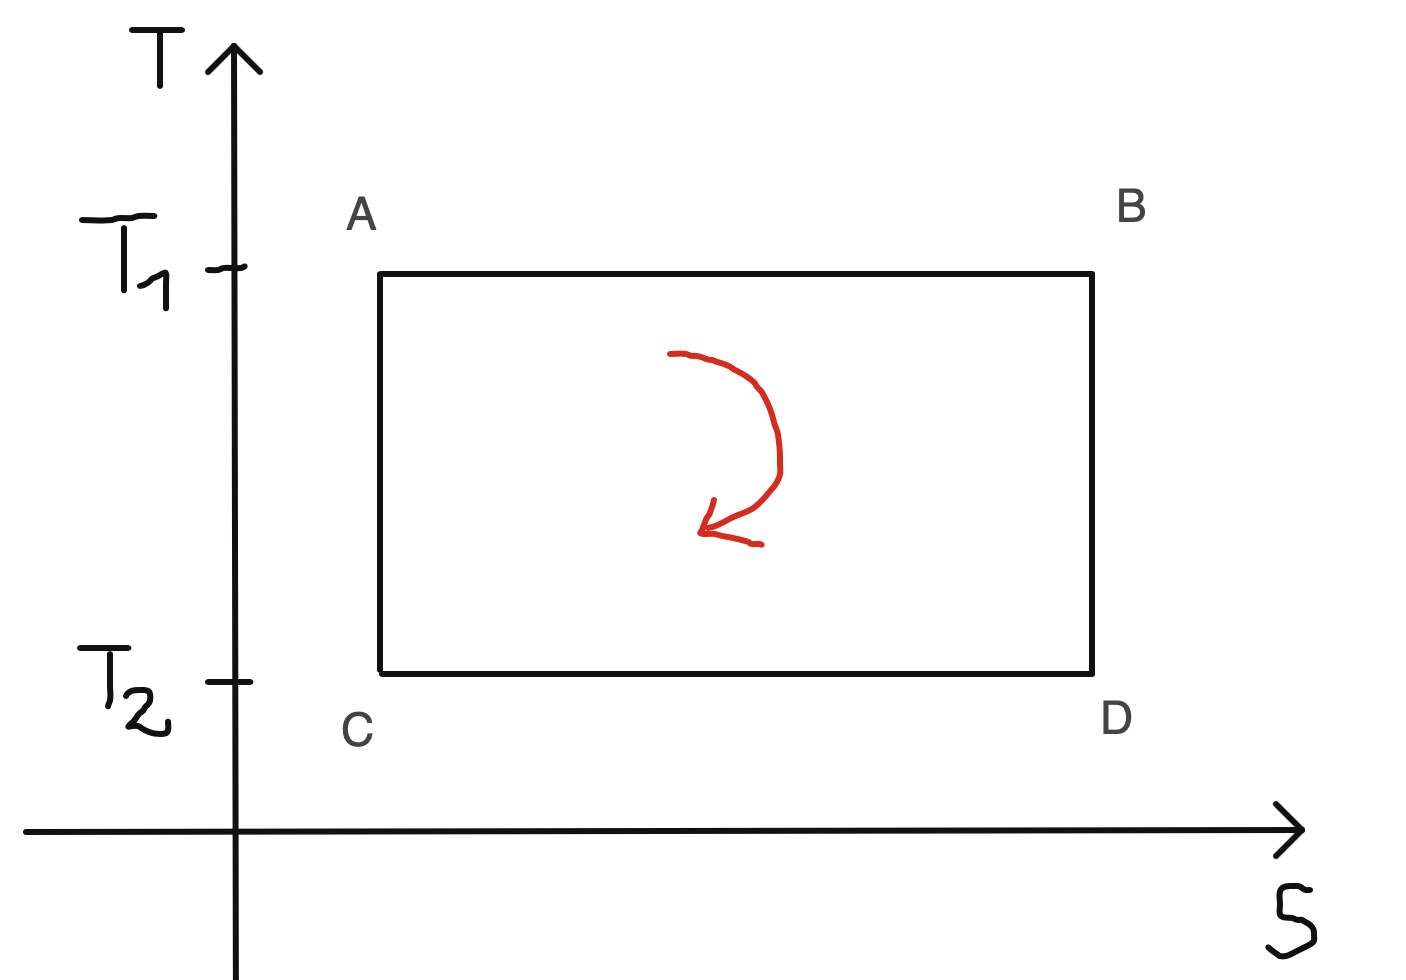
\includegraphics{rys1.png}}
\end{wrapfigure}
Ciepło wymieniane jest w przemianach izotermicznych:
\begin{align}
Q_{\rm{AB}} = \int_A^{B} {\rm \dbar} Q = T_1 \int_A^{B} {\rm d} S = T_1 (S_B-S_A),
\end{align}
oraz 
\begin{align}
Q_{\rm{CD}} = \int_C^{D} {\rm \dbar} Q = T_2 \int_C^{D} {\rm d} S = T_2 (S_D-S_C) = T_2 (S_A-S_B),
\end{align} 
gdzie skorzystaliśmy z równości $S_A=S_D$ oraz $S_B=S_C$ na izentropach.  \\
Wiemy, że na gałęzi $AB$ gaz roboczy pobiera ciepło ze zbiornika, zatem $Q_{\rm {AB}} >0$, natomiast na gałęzi $CD$ gaz oddaje ciepło do chłodnicy, zatem $Q_{\rm {CD}} <0$. Jednocześnie wiemy, że $Q_{\rm {BC}}=0=Q_{\rm {DA}}$.  \\
Zatem sprawność silna Carnota wyznaczmy ze stosunku różnicy ciepła pobranego $\lvert Q_{\rm {AB}} \rvert$ i oddanego $\lvert Q_{\rm {CD}} \rvert$ do ciepła pobranego  $\lvert Q_{\rm {AB} }\rvert$:
\begin{align}
\eta_C = \frac{\lvert Q_{\rm {AB}} \rvert- \lvert Q_{\rm {CD}} \rvert}{\lvert Q_{\rm {AB}} \rvert} = \frac{(T_1 -T_2)(S_A-S_B)}{T_1(S_A-S_B)} = \frac{T_1-T_2}{T_1}= 1 - \frac{T_2}{T_1}.
\end{align}
\\
Powyższą zależność można też wyprowadzić w (trochę) inny sposób.  Skorzystamy tutaj z faktu, iż silnik Carnota składa się z przemian odwracalnych, następujących po sobie w cyklu zamkniętym. Oznacza to, w szczególności, że zmiana entropii na poszczególnych gałęziach cyklu jest równa:
\begin{align}
\Delta S_{\rm AB} = \frac{Q_{\rm AB}}{T_1} , \quad 
\Delta S_{\rm BC} =  0, \quad \Delta S_{\rm CD} = \frac{Q_{\rm CD}}{T_2}, \Delta S_{\rm DA} = 0,
\end{align}
i korzystając z faktu, że entropia jest funkcją stanu (a zatem jej zmiana w cyklu zamkniętym jest równa zero) mamy:
\begin{align}
\Delta S = 0 =  \frac{Q_{\rm AB}}{T_1}  +  \frac{Q_{\rm CD}}{T_2}, \implies  Q_{\rm CD} =- Q_{\rm AB} \frac{T_2}{T_1}.
\end{align}
Ponadto, energia wewnętrzna w cyklu zamkniętym również pozostaje stała,
\begin{align}
\Delta U = \int_{ABCDA}{\rm \dbar}Q + \int_{ABCDA}{\rm \dbar}W  \implies  \int_{ABCDA}{\rm \dbar}W  = -  \int_{ABCDA}{\rm \dbar}Q=\int_{AB}{\rm \dbar}Q + \int_{CD}{\rm \dbar}Q = - \left(1-\frac{T_2}{T_1} \right)\int_{AB} {\rm \dbar}Q ,
\end{align}
Zatem,
\begin{align}
\eta_C= \frac{\lvert \int_{ABCDA}{\rm \dbar}W \rvert}{\int_{AB}{\rm \dbar }Q} = \frac{-\int_{ABCDA}{\rm \dbar}W }{\int_{AB}{\rm \dbar}Q} = 1- \frac{T_2}{T_1}.
\end{align}
Wynik ten nie zależy od rodzaju gazu roboczego!\\
Na koniec udowodnijmy, że sprawność silnika Carnota jest maksymalna. 
W tym celu wyznaczmy zmianę entropii wszechświata. Grzejnik oddaje ciepło $Q_{AB}$, przy czym nie zmienia się jego temperatura $T_1$. Zmiana entropii grzejnika wynosi zatem:
\begin{align}
\Delta S_g = - \frac{|Q_{\rm AB}|}{T_1}.
\end{align}
Chłodnica natomiast pobiera ciepło w stałej temperaturze $T_2$, zatem:
\begin{align}
\Delta S_c=  \frac{|Q_{\rm CD}|}{T_2}.
\end{align}
Zatem całkowita zmiana entropii wynosi:
\begin{align}
\Delta S_{\text{total}} = \Delta S_g + \Delta S_c = - \frac{|Q_{\rm AB}|}{T_1}+ \frac{|Q_{\rm CD}|}{T_2}.
\end{align}
Z drugiej zasady termodynamiki, wiemy, że zmiana entropii jest zawsze nieujemna:
\begin{align}
- \frac{|Q_{\rm AB}|}{T_1}+ \frac{|Q_{\rm CD}|}{T_2} \geq 0.
\end{align}
A stąd mamy:
\begin{align}
\frac{|Q_{\rm CD}|}{T_2}  \geq  \frac{|Q_{\rm AB}|}{T_1}\\
\frac{|Q_{\rm CD}|}{|Q_{\rm AB}|} \geq \frac{T_2}{T_1}\\
1- \frac{|Q_{\rm CD}|}{|Q_{\rm AB}|}  \leq 1 -  \frac{T_2}{T_1}.
\end{align}
Lewa strona powyższej nierówności jest sprawnością dowolnego silnika $\eta$, a strona prawa to sprawność silna Carnota $\eta_C$. Zatem sprawność $\eta_C$ jest sprawnością maksymalną silnika cieplnego.\\
%%%%%%%%%%%%%%%%%%%%%%%%%%%%%%%%%%%%%%%%
\newpage
%%%%%%%%%%%%%%%%%%%%%%%%%%%%%%%%%%%%%%%%
\zadanie
Narysuj we współrzędnych $T-S$ cykl Stirlinga (dwie izotermy, dwie izochory) 
oraz oblicz jego sprawność (z regeneracją i bez).
Porównaj z cyklem Carnota.
\\
\textbf{Rozwiązanie:}
Załóżmy, że gazem roboczym jest gaz doskonały, którego entropia jest równa:
\begin{align}
S =n C_V \ln{T} + nR \ln{V} + S_0. 
\end{align}
W celu narysowania cyklu Stirlinga we współrzędnych $T_S$ potrzebujemy znaleźć równanie izochory w tych współrzędnych. Wiemy, że $V=const$, zatem po prostych przekształceniach otrzymujemy:
\begin{align}
\exp{\frac{S-S_0 - nR \ln{V}}{n C_V}} = T \implies \quad T = \exp{\tilde{S}}.
\end{align}
Dla różnych $V$ otrzymujemy przesunięte eksponenty.\\
\begin{figure}[h!]
\begin{center}
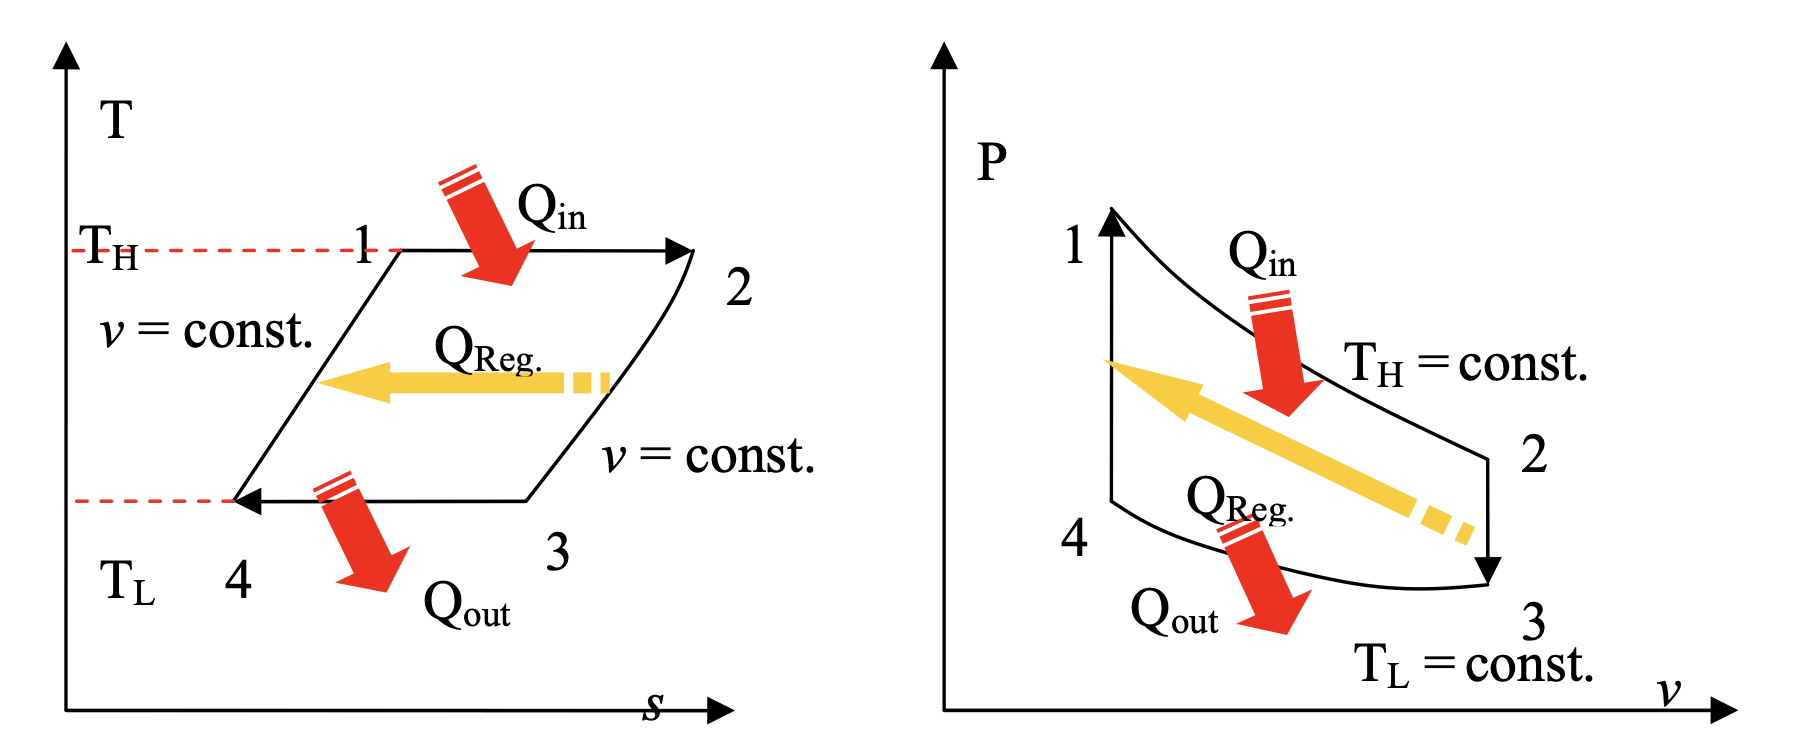
\includegraphics[scale=0.5]{rys3.png}
\caption{Photo credit: $http://www.sfu.ca/~mbahrami/ENSC\%20461/Notes/Stirling\%20Cycle.pdf$}
\end{center}
\end{figure}

Przeanalizujemy bilans ciepła na poszczególnych gałęziach cyklu:
\begin{enumerate}[a)]
\item przemiana $1 \rightarrow 2$ - izoterma $T_H =const.$  (gaz pobiera ciepło z zewnętrznego źródła):
\begin{align}
Q_{\rm 12} =T_H \int_1^2 {\rm d} S = T_H (S_2-S_1)>0,
\end{align}
\item przemiana $2 \rightarrow 3$ - izochora (gaz oddaje ciepło do regeneratora):
\begin{align}
Q_{\rm 23} =n C_V (T_L -T_H)<0,
\end{align}
\item przemiana $3 \rightarrow 4$ - izoterma $T_L=const.$  (gaz oddaje ciepło do zewnętrznego źródła):
\begin{align}
Q_{\rm 34} =T_L \int_3^4 {\rm d} S = T_L (S_4-S_3)<0,
\end{align}
\item przemiana $4 \rightarrow 1$ - izochora (gaz pobiera ciepło z generatora):
\begin{align}
Q_{\rm 41} =n C_V (T_H -T_L)>0,
\end{align}
\end{enumerate}
Z faktu, że gałąź $2\rightarrow 3$ jest izochorą wynika:
\begin{align}
S_2-S_3 = n C_V \ln{\frac{T_H}{T_L}},
\end{align}
Podobnie dla gałęzi $4 \rightarrow 1$:
\begin{align}
S_4-S_1 = n C_V \ln{\frac{T_L}{T_H}},
\end{align}
Stąd:
\begin{align}
S_3-S_2= S_4-S_1 
\end{align}
Ostatecznie sprawność silnika:
\begin{align}
\eta&= \frac{\lvert Q_{12}\rvert + \lvert Q_{\rm 41}\rvert - \lvert Q_{23}\rvert - \lvert Q_{34}\rvert }{\lvert Q_{12}\rvert + \lvert Q_{41}\rvert}\\
&= \frac{ T_H (S_2-S_1) + n C_V (T_H-T_L) - nC_V (T_H-T_L)-T_L(S_3-S_4)}{T_H (S_2-S_1) + n C_V (T_H-T_L) }\\
&= \frac{(T_H-T_L)\Delta S}{n C_V (T_H-T_L)+ T_H \Delta S},
\end{align}
gdzie,
\begin{align}
\Delta S = S_2 -S_1 = n R \ln{\frac{V_2}{V_1}},
\end{align}
stąd:
\begin{align}
\eta &=  \frac{(T_H-T_L)\ln{\frac{V_2}{V_1}}}{ C_V/R (T_H-T_L)+ T_H \ln{\frac{V_2}{V_1}}}.
\end{align}
Jeżeli część $r$ ciepła oddawanego na izochorze $23$ udaje się odzyskać to wtedy $r \lvert Q_{23} \rvert = r \lvert Q_{41} \rvert$,  a ilość ciepła  zmniejsza się do $Q_{23}^{\prime} = (1-r) Q_{23}$ i wtedy:
\begin{align}
\eta_r &=  \frac{(T_H-T_L)\ln{\frac{V_2}{V_1}}}{ \frac{C_V}{R} (T_H-T_L)(1-r)+ T_H \ln{\frac{V_2}{V_1}}}.
\end{align}
Widzimy, że dla $r=1$ sprawność silnika Stirlinga jest taka sama jak sprawność silnika działającego między grzejnikiem o temperaturze $T_1$,  chłodnica o temperaturze $T_2$.

%%%%%%%%%%%%%%%%%%%%%%%%%%%%%%%%%%%%%%%%
\newpage
%%%%%%%%%%%%%%%%%%%%%%%%%%%%%%%%%%%%%%%%
\zadanie
Obliczyć sprawność silnika cieplnego, którego cykl we współrzędnych $T-S$ jest trójkątem
prostokątnym którego podstawa jest zadana przez 
izotermę $T_1$, a wysokość przez adiabatę (między $T_1$ i $T_2$),  trzeci proces domyka trójkąt.
Wynik podać jako funkcję $T_1$ i $T_2$.
\\
\textbf{Rozwiązanie:}


Z faktu, że rozważamy silnik pracuje w cyklu zamkniętym, wynika, że jego energia wewnętrzna się nie zmienia:
\begin{align}
\Delta U = W + Q, \implies W = - Q.
\end{align}
Ciepło dostarczane/odbierane jest do gazu na izotermie $\rm{AB}$ oraz w trakcie przemiany $\rm{CA}$.
Na gałęzi $\rm {AB}$ temperatura gazu roboczego wynosi $T_1$, zatem ciepło wymienione obliczamy jako:
\begin{align}
Q_{\rm AB} = T_1 \int_A^B {\rm d}S = T_1 (S_B - S_A).
\end{align}
Na gałęzi $\rm CA$ temperatura gazu nie jest stała. Zależność $T(S)$ wyznaczymy znajdując równanie prostej, do której należą punkty o współrzędnych $(S_A, T_1 )$ oraz $(S_B, T_2)$. Mamy stąd:
\begin{align}
T(S) &= \frac{T_2 -T_1}{S_B-S_A} S +  T_2 - S_B \frac{T_2 -T_1}{S_B-S_A}\\
&= T_2 + \frac{T_2 -T_1}{S_B-S_A}  (S-S_B)
\end{align}
Ciepło wymienione na tej gałęzi jest równe:
\begin{align}
Q_{\rm {CA}}= \int_C^A T(S) {\rm d} S = T_2 (S_A- S_B) + \frac{1}{2}\frac{T_2- T_1}{S_B-S_A} (S_A-S_B)^2 = \frac{1}{2}(S_A-S_B)(T_2+T_1)
\end{align}
gdzie skorzystaliśmy z faktu, że $S_C=S_B$.\\
Sprawność takiego silnika wynosi:
\begin{align}
\eta = \frac{\lvert Q_{\rm CA} \rvert - \lvert Q_{\rm AB} \rvert }{\lvert Q_{\rm CD} \rvert} = \frac{\frac{1}{2}(S_A-S_B)(T_1+T_2)- T_1(S_A-S_B)}{\frac{1}{2}(S_A-S_B)(T_1+T_2)} = \frac{T_2-T_1}{T_2+T_1}
\end{align}

%%%%%%%%%%%%%%%%%%%%%%%%%%%%%%%%%%%%%%%%
\newpage
%%%%%%%%%%%%%%%%%%%%%%%%%%%%%%%%%%%%%%%%
\zadanie
Zbiornik zawiera $100\,$kg wody o temperaturze $T_1 = 100^\circ$C.
Znajdź maksymalną pracę, jaką może wykonać maszyna cieplna pracująca pomiędzy tym zbiornikiem a otoczeniem o temperaturze $T_2 = 0^\circ$C.
Założyć, że w~trakcie całego procesu rozkład temperatury wewnątrz zbiornika jest jednorodny.\\
\\
\textbf{Rozwiązanie:} Maksymalną pracę silnik wykona operując w cyklu Carnote'a. Rozważmy zatem infinitezymalny cykl Carnote'a, operujący między tempraturami: otoczenia $T_2$ i aktualną temperaturą zbiornika $T$. W związku z tym, że cykl jest infinitezymalny możemy założyć, że w jednym obiegu cyklu pobór temperatury ze zbiornika zachodzi przy stałej temperaturze $T$.

Praca wykonana w cyklu wynika z równania na sprawność silnika operujacego w cyklu Carnote'a:
\begin{equation}
dw = \left(1-\frac{T_2}{T}\right) dq,
\end{equation} 
gdzie $dq$ jest ciepłem pobranym w cyklu. \textbf{Zwróćmy uwagę, że $dq$ i $dw$ nie mają dużo wspólnego z termodynamicznymi formami ciepła i pracy.} Ciepło wymienione można połączyć ze zmianą temperatury:
\begin{equation}
dq = -m c d T.
\end{equation}
Możemy scałkować $dw$ od temperatury $T_1$ do $T_2$ (kiedy zbiornik ma temperaturę otoczenia), aby otrzymać całkowitą pracę:
\begin{align}
W &= \int dw = \int_0^{mc (T_1-T_2)} \left(1-\frac{T_2}{T}\right) dq = \int_{T_1}^{T_2} \left(1-\frac{T_2}{T}\right) (-m c dT) \\
&= mc \int_{T_2}^{T_1}\left(1-\frac{T_2}{T}\right) dT = mc \left(T_1-T_2 - T_2 \log\left(\frac{T_1}{T_2}\right)\right) = 6.21\; {\rm MJ}.
\end{align} 
Możemy zauważyć, że $mc \left(T_1-T_2\right)$ to ciepło przekazane w procesie, a ostatni wyraz to straty będace konsekwencją ograniczonej efektywności silnika. 

%%%%%%%%%%%%%%%%%%%%%%%%%%%%%%%%%%%%%%%%
\newpage
%%%%%%%%%%%%%%%%%%%%%%%%%%%%%%%%%%%%%%%%
\zadanie
Dwa zbiorniki zawierają po $100\,$kg wody każdy.
W jednym woda ma temperaturę $T_1=100^\circ$C,
zaś w drugim $T_2 = 0^\circ$C. Jaką maksymalna pracę można wykonać
używając jednego zbiornika jako grzejnika a drugiego jako chłodnicy?
Ciepło właściwe wody wynosi $c_w=4200\,{\rm J/(kg\, K)}$.
\\
\textbf{Rozwiązanie:}
Wyznaczmy zmianę entropii zbiorników:
\begin{align}
\Delta S_1 = \int \frac{{\rm \dbar}Q}{T} = mc \int_{T_1}^{T_k}\frac{ {\rm d}T}{T} = mc \ln{\frac{T_k}{T_1}} 
\end{align}
oraz
\begin{align}
\Delta S_2 = \int \frac{{\rm \dbar}Q}{T} = mc \int_{T_2}^{T_k}\frac{ {\rm d}T}{T} = mc \ln{\frac{T_k}{T_2}}. 
\end{align}
Maksymalną pracę wykonamy, gdy całkowita entropia się nie zmieni tJ.:
\begin{align}
\Delta S = \Delta S_1 + \Delta S_2 = mc \ln{\frac{T_k^2}{T_1 T_2}}=0.
\end{align}
a stąd:
\begin{align}
\frac{T_K^2}{T_1T_2}=1, \implies T_k = \sqrt{T_1 T_2}.
\end{align}
Praca wykona przez maszynę obliczamy jako:
\begin{align}
W = \lvert Q_1 \rvert  -\lvert  Q_2 \rvert =mc \left( T_1 +T_2 - 2 T_k\right)
\end{align}
Po podstawieniu danych liczbowych otrzymujemy:
\begin{align}
W= 3.27\; {\rm MJ}
\end{align}



% An example of figure placement:
%\begin{wrapfigure}[13]{r}{0.4\linewidth}\vspace{3mm}
%\resizebox{\linewidth}{!}{\includegraphics{NAZWA.png}}
%\end{wrapfigure}
%\zaddom


\end{document}

